\section{System Architecture}
\label{sec:arch}

The complete pipeline created for this project breaks down into five sequential stages, shown in \fref{fig:pipeline}: (1) data collection, in which page images of the newspaper are obtained; (2) page preprocessing, in which each page is cleaned; (3) article segmentation and OCR, in which every page is split into separate, correctly ordered articles which are then read by Tesseract, cleaned and filtered; (4) analysis, in which three sentiment methods and the BERTopic topic model are run in parallel on the same articles; and (5) integration and evaluation, in which the results are joined and analysed by topic, page type and time, and the sentiment methods are compared with each other and with human labels.

The first phase of the project (previous semester) covered the text-based part of this chain: OCR text of newspaper pages was cleaned and given to three topic models, LSA, LDA and BERTopic (Section~\ref{sec:phase1}). The second phase, which is the main subject of this chapter, added automatic page acquisition, article segmentation, the three sentiment methods and the evaluation methodology, and applied the whole chain to a full year of a newspaper.

\begin{figure}[t]
\centering
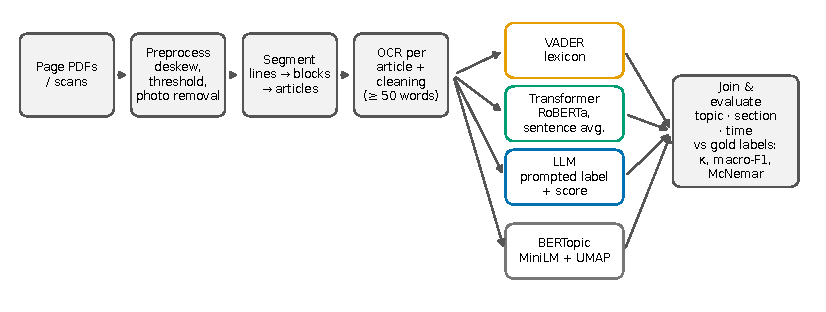
\includegraphics[width=\textwidth]{Ch03/fig1_pipeline.pdf}
\caption{Pipeline of the proposed system. Page images are cleaned and segmented into articles; each article is OCR'd, cleaned and filtered to at least 50 words; VADER, the RoBERTa transformer, Claude Haiku (prompted) and BERTopic then run in parallel, and their results are joined and evaluated by topic, section and time and against human (gold) labels.}
\label{fig:pipeline}
\end{figure}

Every stage stores its result on disk page by page, together with a version number of the processing logic. A stopped run can therefore be resumed, a page is recomputed only when the logic changed, and the original page images are only ever read, never modified.

\section{Data Collection}
\label{sec:collect}

\subsection{Source and Coverage}
The corpus consists of The Indian Express, Jaipur edition, for the whole of 2025 (1 January to 31 December). Two pages of each issue were chosen: the front page, which shows what the newspaper treats as the most important news of the day, and the editorial page, which carries the newspaper's own opinion and invited commentary. The front page is collected for every issue and the editorial page for every issue from Monday to Saturday, because there is no editorial page in the Sunday edition. In 2025 the e-paper listed 358 issues (seven calendar days have no issue), 52 of them Sunday issues, so the target was 358 front pages and 306 editorial pages.

\subsection{Collection from the E-paper}
The first week of January was downloaded by hand as PDF pages and used for the development of the pipeline. For the full year this was replaced by an automatic collector, because downloading more than six hundred pages by hand is neither practical nor reproducible. The collector works with the subscriber's own login to the e-paper and follows the same requests as the web reader:

\begin{enumerate}
\item The user logs in once in a browser window, and the session token is saved locally (the program never sees or stores the password). The token is exchanged for a bearer token that authorises the e-paper's data interfaces.
\item For each month, the issue list of the Jaipur edition is requested, giving the issue identifier of each date.
\item For each issue, a page manifest is requested. It lists, for every page, several resolution levels; each level is a grid of image tiles, a JPEG background tile and a transparent PNG tile that carries the text and line art. A small header image of each page is also listed.
\item The tiles of the chosen page are downloaded (the image server rejects requests that carry the authorisation header, so they are fetched in a separate, clean session) and stitched together: the background tiles are pasted and the text tiles are alpha-composited on top, giving one full-page image.
\end{enumerate}

The highest available resolution is used. For the issues from 1 January to 25 March, only the 1600$\times$2226 pixel level was available (150 pages); from 26 March onwards the 2400$\times$3339 pixel level was available (513 pages). Requests are made one at a time with fixed pauses (1.0\,s between requests, 0.3\,s between tiles, 2\,s between pages and 4\,s between days), and finished days are recorded in a manifest file, so a stopped run resumes where it ended. The e-paper also offers a single-page PDF download, but it asks for a CAPTCHA each time; we deliberately do not attempt to get around it and use only the image tiles that the reader itself displays.

\subsection{Identifying the Front and the Editorial Page}
The number and position of pages differ from issue to issue, and the paper is often wrapped in a full-page advertisement (a ``jacket''), so the front page is not always page 1. Pages are therefore identified by their content. The header image of each page is OCR'd twice (as it is, and enlarged with increased contrast) and matched with regular expressions.
\begin{itemize}
\item \textbf{Front page}: the first page that is not an advertisement and whose next page is headed ``The Second Page'' (found this way for 338 of the 358 issues); otherwise the first non-advertisement page with the newspaper's masthead; otherwise the first non-advertisement page.
\item \textbf{Editorial page}: the page whose header image or whose own title strip reads ``The Editorial Page'' or carries the fixed ``Wordly Wise'' column (297 of the 305 editorial pages), otherwise the page directly before ``The Ideas Page'' (8 pages). The front page is never accepted as the editorial page.
\end{itemize}

\subsection{Verification of the Collected Pages}
\label{sec:verify}
A verification pass after the first full download showed why the second rule matters. From November 2025 the front page carries a teaser line such as ``The Editorial Page: We saw the IndiGo meltdown\ldots'' at its top, which the first version of the detector took for the editorial page: on 23 days the front page had been saved a second time as the editorial page, on 5 further days another page had been taken, and on 21 days no editorial page was found. The detector was changed to read the title strip of each page itself, to exclude the front page and to ignore page 1, and a separate verification program was added. It OCRs the top of every saved editorial page, and reports files whose title is not ``The Editorial Page'' (or ``Wordly Wise'') or that are identical to the front page of the same day. The 28 wrong files were moved to a separate folder instead of being deleted, and the affected days were downloaded again. After the correction, all 305 editorial files passed the check; only one editorial page (23 December) could not be found.

\subsection{Ethical and Legal Considerations}
The page images are copyrighted material that was obtained through a paid subscription, solely for non-commercial academic research. The images and full article texts are not redistributed. This report only presents derived statistics, short headline fragments for illustration and charts. Access to the e-paper is rate limited and authenticated, and no protection mechanism (such as the CAPTCHA) is circumvented.

\section{Page Preprocessing}
\label{sec:preprocess}

Each page image is brought to a common working resolution of 4500 pixels width (about 360 dpi relative to the printed page), at which body text is 30--35 pixels per em, the range that Tesseract handles best. Images of lower resolution are enlarged by cubic interpolation, PDF pages are rendered at this width. The following steps then prepare the page for OCR.

\begin{enumerate}
\item \textbf{Deskew.} A projection-profile method estimates the page rotation: the page is rotated through candidate angles (coarse steps of $0.25^{\circ}$ within $\pm 5^{\circ}$, then fine steps of $0.05^{\circ}$), and the angle at which the row profile of the ink is sharpest, that is, at which text lines are horizontal, is kept. The e-paper pages were already almost straight (mean absolute skew $0.05^{\circ}$), but scans of printed pages are not.
\item \textbf{Photograph removal.} Printed text is almost pure black on white, so a window of text has few mid-grey pixels, while continuous-tone photographs and halftone screens have many. Windows of about 60 pixels in which more than 40\% of the pixels are mid-grey, more than 70\% are non-white or more than half are strongly coloured are marked as photograph candidates; only large, roughly rectangular regions are kept (at least 150 pixels on each side), which excludes coloured headlines and kickers. The regions are blanked out before OCR (3,111 photographs were removed in total). The regions are kept, because they are used later to recognise captions and to ignore rules that belong to photographs.
\item \textbf{Binarisation.} The grey page is converted to black and white with Sauvola's local adaptive threshold \cite{sauvola2000}, $T(x,y) = m(x,y)\left[1 + k\left(\frac{s(x,y)}{R} - 1\right)\right]$, where $m$ and $s$ are the mean and standard deviation of the grey values in a $51\times 51$ pixel window, $R = 128$ is the dynamic range of the standard deviation (the usual default) and $k = 0.2$. A local threshold copes with the uneven ink and paper tone that a single global threshold cannot.
\item \textbf{Removal of printed rules.} Long thin horizontal and vertical lines (the rules between columns and stories) are found with morphological opening, including dotted and dashed rules, which are found as long rows of tiny flat components. Their pixels are erased so they do not disturb OCR, but their positions are kept: they separate columns and articles in the segmentation step.
\end{enumerate}

\section{Article Segmentation}
\label{sec:segment}

The step that is least covered by OCR software is the division of the page into articles. Tesseract's page-level layout mode returns text blocks, but on a newspaper page it merges neighbouring columns and cannot tell a headline from a caption. We therefore built a rule-based layout analyser that uses Tesseract only to find text lines and their heights, and takes the remaining decisions from the typography of the page. Four ideas make it work: type size relative to the body text, rules and whitespace as separators, headlines as the anchor of an article, and the reading order of columns. The main steps are listed below; the thresholds are collected in \tref{tab:params}.

\subsection{Lines and Blocks}
Tesseract in page-segmentation mode 3 (fully automatic layout) returns lines with their bounding boxes and confidences. Lines that cross a vertical rule are cut at the rule, and headline lines are also cut at unusually large gaps between words, because headlines of two neighbouring stories often sit on the same line. Headlines in very large type that the page-level pass skips are recovered by a second pass. A line is then chained to the block directly above it if the two overlap horizontally, have a similar type size (height ratio between 0.67 and 1.5), are close together and are not separated by a horizontal rule.

\subsection{Type-size Classes}
The height $H$ of body text is measured on each page as the median of the line heights weighted by the number of words in a line, so that the many lines of running text decide it. Every block is then classified relative to $H$: \emph{headline} (line height at least $1.75H$), \emph{deck} (kicker or stand-first, at least $1.25H$), \emph{small print} (below $0.8H$, for credits, tables and captions) or \emph{body}. Because the classes are relative, the same rules work at all the resolutions at which pages were collected. A very narrow block (for example a rotated label such as ``EXPLAINED'') is treated as small print, not as a headline.

\subsection{Page Furniture}
Blocks that are not articles are marked and left out: the masthead (found in the top 22\% of the page), the footer strip (the bottom 2.5\%), text inside photographs, and photo captions (short blocks of at most four lines directly below a photograph that overlap it horizontally by at least half).

\subsection{Headline Groups and Article Assignment}
Adjacent headline and deck blocks that are aligned within a distance of $4H$ form a headline group (a kicker, a headline and its stand-first); a deck-only group and a byline are folded into the headline group above. Each body block is then joined to what sits directly above it in its column, either a headline group or a body block that was already assigned, but never across a horizontal rule. Each member of a headline group has its own anchor, so a chart title in the middle of a story does not stretch the headline box of that story. A second pass assigns text columns that no headline reached (typical on the editorial page, where a byline interrupts the column) by ignoring rules when nothing lies in between.

\subsection{Reading Order and Page Type}
The blocks of an article are put in reading order: columns from left to right, and inside each column from top to bottom. The page type (front, editorial or other) is decided from the page content, with the file name used as a check.

\subsection{Reliability Flags}
Because no human inspects every page, the pipeline marks pages whose result looks suspect, so that they can be reviewed or excluded. A page is flagged when it kept fewer than two or more than twenty articles, when one article holds more than 60\% of the text of the page (a likely merge), when more than 25\% of the body text had no headline above it, when the mean OCR confidence is below 75, or when the skew is larger than $2^{\circ}$. For every page the report lists the number of candidate articles, the numbers dropped as too short or as duplicates, the mean OCR confidence and the flags. Overlay images that draw the article boxes on each page are also written, to make the visual checking of any page quick.

\begin{table}[t]
\centering
\caption{Main parameters of the page processing stage}
\label{tab:params}
\small
\setlength{\tabcolsep}{5pt}
\begin{tabular}{@{}l p{6.5cm} l@{}}
\toprule
\textbf{Step} & \textbf{Parameter} & \textbf{Value}\\
\midrule
Rendering      & Working width of the page                           & 4500 px\\
Deskew         & Search range (coarse step, fine step)               & $\pm 5^{\circ}$ ($0.25^{\circ}$, $0.05^{\circ}$)\\
Photographs    & Mid-tone share / non-white share of a window        & 40\% / 70\%\\
Binarisation   & Sauvola window size, $k$                            & 51 px, 0.2\\
Rules          & Minimum length / maximum thickness                  & 300 px / 12 px\\
Layout         & Tesseract mode for lines / for article blocks       & PSM 3 / PSM 6 (OEM 1)\\
Size classes   & Headline / deck / small, relative to body height $H$ & $\ge 1.75H$ / $\ge 1.25H$ / $<0.8H$\\
Furniture      & Masthead zone / footer zone (share of page height)  & 22\% / 2.5\%\\
Articles       & Minimum length of an article                        & 50 words\\
Duplicates     & Pull quote repeating $\ge 60\%$ of another block    & dropped\\
\bottomrule
\end{tabular}
\end{table}

\section{Article OCR and Text Cleaning}
\label{sec:ocr}

Each article is read separately: the headline and the deck boxes are cropped and read first, followed by the body blocks in reading order, all with Tesseract (LSTM engine) in page-segmentation mode 6 (a single uniform block of text), which is more reliable than the page-level mode on a crop that is known to contain text. Tesseract's per-word confidences are kept and averaged per article. A pull quote, that is a block that repeats most of the text of another block of the same article, is detected by word-sequence overlap (60\% or more) and dropped.

The raw text is then cleaned in the following steps.
\begin{itemize}
\item \textbf{Character fixes}: typographic ligatures, curly quotation marks and dashes are replaced by plain characters.
\item \textbf{Dehyphenation}: a word broken across a line (``govern-'' / ``ment'') is joined only when the joined word is in a dictionary or has been seen unbroken elsewhere on the same page; a likely real compound (``long-term'') keeps its hyphen.
\item \textbf{Removal of page furniture and junk}: ``Continued on page\ldots'' lines, stand-alone page numbers, web addresses of the newspaper, and lines that consist mostly of symbols or of one- and two-character fragments (noise from graphics) are dropped. Lines for which Tesseract's own confidence is below 30 are also treated as noise already in the layout step.
\item \textbf{Bylines}: leading author lines and datelines (all capitals, or of the form ``NEW DELHI, DECEMBER 31'') are removed from the text and stored separately.
\item \textbf{Length filter}: articles with fewer than 50 words are removed; they are mostly captions, teasers and brief items, which carry too little text for a stable judgement of tone.
\item \textbf{Sentence splitting} for the sentence-level sentiment methods: a rule-based splitter that cuts after sentence punctuation, does not cut after common abbreviations (``Dr.'', ``Mr.'', ``No.'') and drops fragments shorter than three words.
\end{itemize}
Only the part of a front-page story that is printed on the front page is analysed; the continuation on an inside page is not followed.

\section{Sentiment Analysis}
\label{sec:sentiment}

\subsection{Definition and Output}
Sentiment is defined as the \emph{overall tone of the text} on the scale negative -- neutral -- positive. It is not the author's personal opinion, and it is not the reaction of the reader. A report of a violent event is negative in this sense because its content is harmful, and a report of a scientific achievement is positive. Every method returns for each article a label from \{negative, neutral, positive\} and a score between $-1$ (very negative) and $+1$ (very positive). When the sentiment of a group of articles is summarised, we use the mean score and the \emph{net sentiment}
\begin{equation}
N = \frac{n_{\mathrm{pos}} - n_{\mathrm{neg}}}{n},
\end{equation}
the share of positive articles minus the share of negative articles of the group, which lies in $[-1, 1]$ and is easy to compare between methods.

\subsection{Method 1: VADER (Lexicon)}
Each sentence $s$ of the article is scored with the VADER compound score $c(s)\in[-1,1]$ \cite{hutto2014}. The article score is the mean over its sentences,
\begin{equation}
v = \frac{1}{|S|}\sum_{s\in S} c(s),
\end{equation}
and the label is \emph{positive} if $v \ge 0.05$, \emph{negative} if $v \le -0.05$ and \emph{neutral} otherwise, which are the thresholds recommended by the authors of VADER.

\subsection{Method 2: RoBERTa Transformer}
The model \texttt{cardiffnlp/twitter-roberta-base-sentiment-latest} \cite{loureiro2022,barbieri2020} classifies a text as negative, neutral or positive. Because RoBERTa can read at most 512 tokens and about one article in five is longer than that (\fref{fig:corpus} in Chapter~4), each sentence is classified separately and the probabilities are averaged. For the sentences $s \in S$ with class probabilities $\mathbf p_s = (p^{-}_s, p^{0}_s, p^{+}_s)$, the article probabilities are $\bar{\mathbf p} = \frac{1}{|S|}\sum_s \mathbf p_s$, the score is
\begin{equation}
t = \bar p^{+} - \bar p^{-},
\end{equation}
and the label is the class with the largest average probability. The model is run with the Hugging Face Transformers library \cite{wolf2020} on the Apple GPU of the development machine. The headline is also scored separately by the same model (headline score), because a headline is one sentence that can differ in tone from the story below it.

\subsection{Method 3: Claude Haiku (Large Language Model)}
The third method asks a large language model to judge the whole article. The model is Claude Haiku (version \texttt{claude-haiku-5-5}), the smallest and cheapest model of the Claude family \cite{anthropic2026}; only a Haiku model is allowed in the program for this task. Each request contains the following.
\begin{itemize}
\item A system instruction that makes the model a careful media analyst that answers only in JSON.
\item Written definitions of the three classes: \emph{positive} means that the overall tone is favourable, hopeful or that good news and progress are reported; \emph{negative} means a critical or alarming tone, or reports of conflict, harm, failure or bad news; \emph{neutral} means mainly factual or balanced reporting without a clear slant. The model is told to judge the tone of the text itself and not whether it agrees with it, and that the text comes from OCR and may contain small errors, which should be ignored.
\item The headline (or ``(none)'' if no headline was detected) and the full article text. No article in the corpus reaches the safety cap of 4,000 words, so none was shortened.
\end{itemize}
The answer is requested as a structured output with three fields: \texttt{label}, one of the three classes; \texttt{score}, a number in $[-1,1]$; and \texttt{reason}, at most 20 words. The reasoning effort is set to ``low'', since this is a simple classification task. Four requests are run in parallel, failed requests are retried, and every answer is written to a cache file keyed by a hash of the model name, the headline and the text. A stopped run therefore resumes without paying for the same article twice, and the published results can be reproduced exactly from the cache. Scoring the whole year cost in the order of one to two US dollars.

\begin{table}[t]
\centering
\caption{The three sentiment methods compared in this work}
\label{tab:methods}
\small
\setlength{\tabcolsep}{4pt}
\begin{tabular}{@{}p{2.6cm} p{3.4cm} p{3.4cm} p{3.4cm}@{}}
\toprule
 & \textbf{VADER} & \textbf{RoBERTa transformer} & \textbf{Claude Haiku}\\
\midrule
Type & Word list with rules & Fine-tuned neural classifier & Prompted language model\\
Unit scored & Each sentence, averaged & Each sentence, averaged & Whole article at once\\
Score & Compound, $-1$ to $+1$ & $\bar p^{+} - \bar p^{-}$ & Number given by the model\\
Label rule & $\ge 0.05$ / $\le -0.05$ thresholds & Largest average probability & Chosen by the model\\
Training data & Human-rated lexicon & About 124M tweets, then TweetEval & General (not task specific)\\
Output explained & Word valences & Probabilities & One-line reason\\
Cost & None & None (local GPU) & Small, per request\\
\bottomrule
\end{tabular}
\end{table}

\section{Topic Modeling of the Full Year}
\label{sec:topics}

BERTopic was selected in Phase I (Section~\ref{sec:phase1}) and is used for the year-long corpus. The pipeline of \cite{grootendorst2022} is applied to the cleaned article texts, with the following settings.
\begin{enumerate}
\item \textbf{Embeddings}: each article is embedded with the sentence transformer \texttt{all-MiniLM-L6-v2} \cite{wang2020,reimers2019}, giving a vector of 384 numbers.
\item \textbf{Dimension reduction}: UMAP \cite{mcinnes2018} with 15 neighbours, 5 output dimensions, minimum distance 0 and the cosine metric.
\item \textbf{Clustering}: HDBSCAN \cite{campello2013} with minimum cluster size $\max(15, \lfloor n/110\rfloor) = 51$ for the $n = 5{,}648$ articles, minimum samples 10 and the excess-of-mass cluster selection. These values were chosen after trying several settings: the Phase~I setting ($n/50$ with minimum samples 2) merged almost the whole year into two topics, and much smaller clusters gave 40--60 very fine topics. The chosen setting gives 18 topics, the largest of which holds 14\% of the articles.
\item \textbf{Outliers}: HDBSCAN first leaves a large share of the articles (2,066 of 5,648, 37\%) in its noise class. Each of them is assigned to the topic whose centroid is closest in embedding space, so that every article belongs to a topic and sentiment can be computed for all articles.
\item \textbf{Topic words}: c-TF-IDF over unigrams and bigrams, with a stop-word list that is extended by newspaper vocabulary (``said'', ``according'', ``told'', names of months and days, ``page'', ``continued'', and so on), gives the words that distinguish a topic from all other topics. The weight of a term $t$ in topic $c$ is
\begin{equation}
W_{t,c} = \mathrm{tf}_{t,c}\cdot \log\left(1 + \frac{A}{\mathrm{tf}_t}\right),
\end{equation}
where $\mathrm{tf}_{t,c}$ is the frequency of $t$ in the merged document of topic $c$, $\mathrm{tf}_t$ its frequency over all topics and $A$ the average number of words per topic. The label of a topic is made of its four top words.
\end{enumerate}
The pipeline has fallbacks for small corpora, which are used when it is applied to a short period: below 500 articles HDBSCAN is replaced by $k$-means, with $k \in [5,15]$ chosen by the silhouette score \cite{rousseeuw1987}, and below 100 articles LDA is used, with the number of topics chosen by UMass coherence \cite{mimno2011}. These fallbacks were not needed for the year-long corpus.

\section{Evaluation Methodology}
\label{sec:eval}

\subsection{Agreement Between the Methods}
The three methods are first compared with each other on all articles, without any human label. For each pair we report the share of articles with the same label, Cohen's $\kappa$ \cite{cohen1960}, which corrects the agreement for chance,
\begin{equation}
\kappa = \frac{p_o - p_e}{1 - p_e},
\end{equation}
where $p_o$ is the observed agreement and $p_e$ the agreement expected by chance from the label frequencies of the two methods, and Spearman's rank correlation $\rho$ of the scores \cite{spearman1904}, which asks whether two methods rank the articles in the same order even if they draw the class boundaries in different places. The $\kappa$ values are read with the usual scale of Landis and Koch \cite{landis1977}: below 0.2 slight, 0.2--0.4 fair, 0.4--0.6 moderate agreement.

\subsection{Hand-labelled Sample}
Agreement between methods does not show which of them is right, so the methods are compared with human judgement. A random sample of 50 articles was exported to a spreadsheet from the first-week corpus (PDF pages of 1--7 January), with the predictions of all methods hidden so that they could not influence the human annotator, and the annotator filled in one label per article using the same definitions as in the prompt of the language model. Two articles could not be labelled, so 48 are used. The following measures are reported for each method against these labels:
\begin{itemize}
\item \textbf{accuracy}, with a 95\% Wilson confidence interval \cite{wilson1927};
\item \textbf{macro-F1}, the unweighted mean of the F1 scores of the three classes, $\mathrm{F1}_{\mathrm{macro}} = \frac{1}{3}\sum_{c} \mathrm{F1}_c$, which is not rewarded for always predicting the biggest class;
\item Cohen's $\kappa$, with the baseline ``always answer neutral'' for comparison;
\item an exact McNemar test \cite{mcnemar1947} for each pair of methods, which uses only the articles on which exactly one of the two is right: if $b$ and $c$ are the numbers of articles on which only the first or only the second method is right, the two-sided $p$-value is $\min\left\{1,\; 2\sum_{i=0}^{\min(b,c)}\binom{b+c}{i}2^{-(b+c)}\right\}$;
\item confusion matrices.
\end{itemize}
Confidence intervals of $\kappa$ and macro-F1 are obtained by bootstrap resampling \cite{efron1979}.

\subsection{Group Summaries}
Sentiment is summarised by topic, page type, month and day. For every group the pipeline stores the number of articles, the mean score with a 95\% confidence interval ($\bar x \pm 1.96\,s/\sqrt{n}$), the label shares and the net sentiment, for each of the three methods, in tables that can be re-read in any later analysis. The differences between the front page and the editorial page are tested with the Mann--Whitney $U$ test on the scores and the $\chi^2$ test on the labels, and the differences between months with the Kruskal--Wallis test and the $\chi^2$ test. Daily values are shown with a 7-day rolling mean, weighted by the number of articles.

\section{Implementation}
\label{sec:implementation}

The system is written in Python 3.11 as a command-line program with a small number of modules: page discovery and rendering, preprocessing (OpenCV \cite{bradski2000}, scikit-image \cite{vanderwalt2014}), layout analysis, OCR (Tesseract 5 through \texttt{pytesseract}), text cleaning, sentiment (Transformers \cite{wolf2020}, \texttt{vaderSentiment} and the Anthropic software development kit), topic modeling (BERTopic 0.16, UMAP, HDBSCAN, scikit-learn \cite{pedregosa2011}), summaries, charts and the evaluation of the labels. The collector for the e-paper is a separate program. All settings, including the thresholds in \tref{tab:params}, are collected in a single configuration file. The exact versions of all libraries are fixed in a requirements file, and the random seed is fixed (42), so a repeated run gives the same results.

The program is controlled by a few options (input folder, force recomputation, choice of topic method, choice and model of the language model, switching the comparison off). The work was done on a laptop with an Apple M-series processor. OCR and segmentation took roughly half a minute per page, and the rest of the steps (sentiment of the two local methods, embeddings and clustering) took a few minutes for the whole corpus. The cost of the language model was small (Section~\ref{sec:sentiment}), and it can be replaced by switching the option off, in which case the other two methods and the topics are still computed.
